% Created by tikzDevice version 0.10.1 on 2016-09-09 15:11:32
% !TEX encoding = UTF-8 Unicode
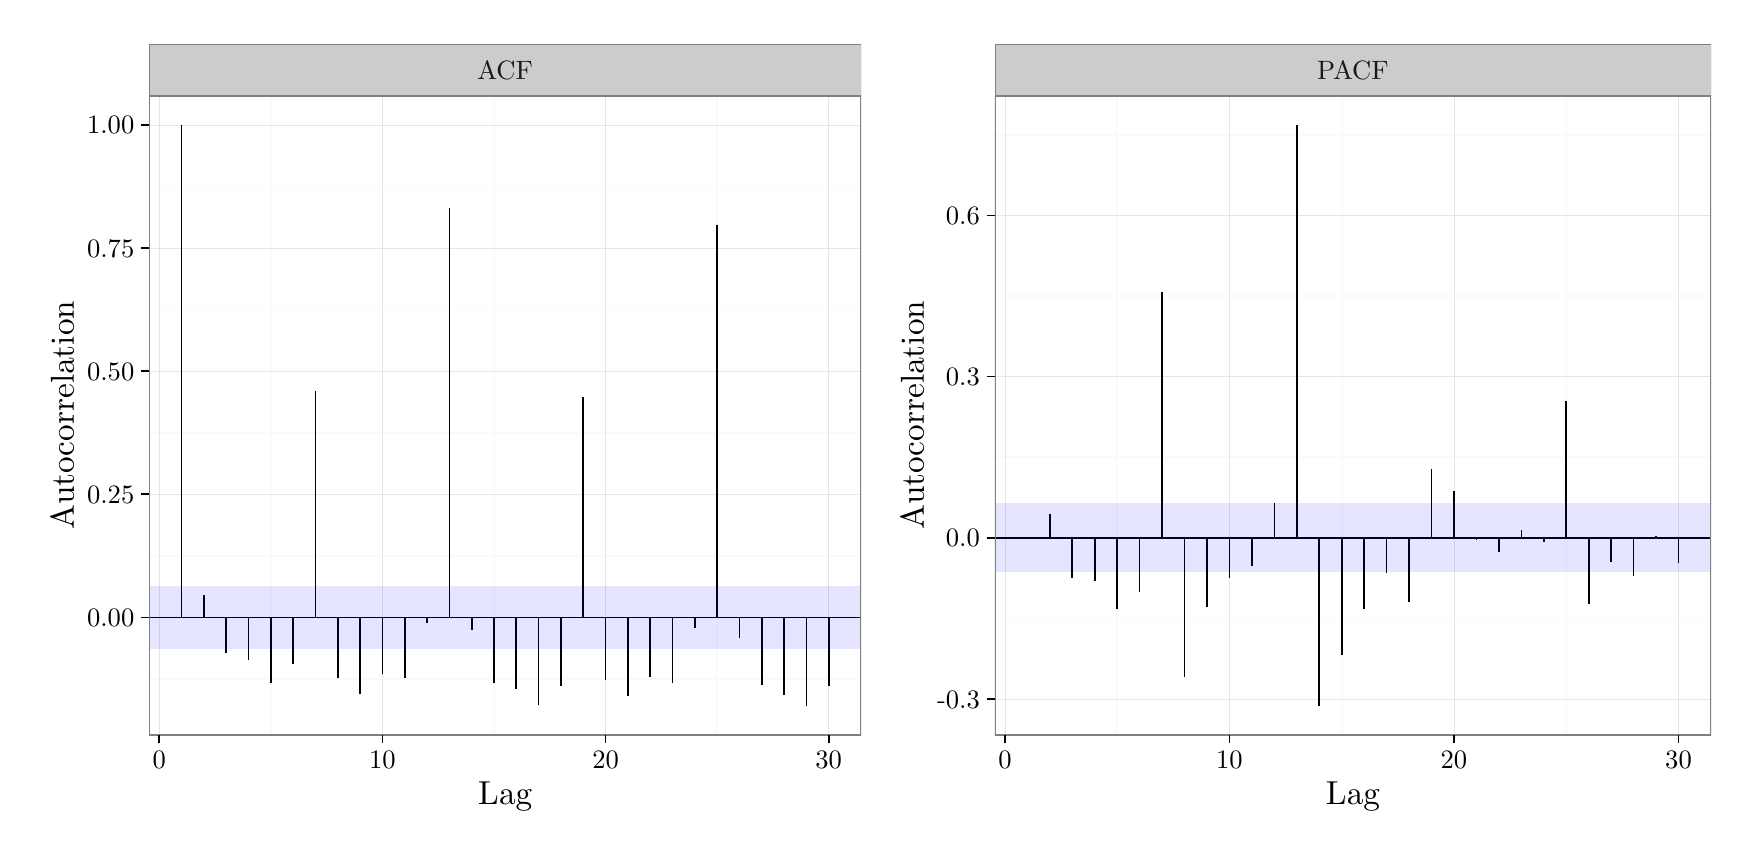
\begin{tikzpicture}[x=1pt,y=1pt]
\definecolor{fillColor}{RGB}{255,255,255}
\path[use as bounding box,fill=fillColor,fill opacity=0.00] (0,0) rectangle (614.29,289.08);
\begin{scope}
\path[clip] (  0.00,  0.00) rectangle (307.15,289.08);
\definecolor{drawColor}{RGB}{255,255,255}
\definecolor{fillColor}{RGB}{255,255,255}

\path[draw=drawColor,line width= 0.6pt,line join=round,line cap=round,fill=fillColor] ( -0.00,  0.00) rectangle (307.15,289.08);
\end{scope}
\begin{scope}
\path[clip] ( 43.93, 33.48) rectangle (301.15,264.47);
\definecolor{fillColor}{RGB}{255,255,255}

\path[fill=fillColor] ( 43.93, 33.48) rectangle (301.15,264.47);
\definecolor{drawColor}{gray}{0.98}

\path[draw=drawColor,line width= 0.6pt,line join=round] ( 43.93, 53.71) --
	(301.15, 53.71);

\path[draw=drawColor,line width= 0.6pt,line join=round] ( 43.93, 98.21) --
	(301.15, 98.21);

\path[draw=drawColor,line width= 0.6pt,line join=round] ( 43.93,142.71) --
	(301.15,142.71);

\path[draw=drawColor,line width= 0.6pt,line join=round] ( 43.93,187.22) --
	(301.15,187.22);

\path[draw=drawColor,line width= 0.6pt,line join=round] ( 43.93,231.72) --
	(301.15,231.72);

\path[draw=drawColor,line width= 0.6pt,line join=round] ( 87.87, 33.48) --
	( 87.87,264.47);

\path[draw=drawColor,line width= 0.6pt,line join=round] (168.51, 33.48) --
	(168.51,264.47);

\path[draw=drawColor,line width= 0.6pt,line join=round] (249.14, 33.48) --
	(249.14,264.47);
\definecolor{drawColor}{gray}{0.90}

\path[draw=drawColor,line width= 0.2pt,line join=round] ( 43.93, 75.96) --
	(301.15, 75.96);

\path[draw=drawColor,line width= 0.2pt,line join=round] ( 43.93,120.46) --
	(301.15,120.46);

\path[draw=drawColor,line width= 0.2pt,line join=round] ( 43.93,164.96) --
	(301.15,164.96);

\path[draw=drawColor,line width= 0.2pt,line join=round] ( 43.93,209.47) --
	(301.15,209.47);

\path[draw=drawColor,line width= 0.2pt,line join=round] ( 43.93,253.97) --
	(301.15,253.97);

\path[draw=drawColor,line width= 0.2pt,line join=round] ( 47.56, 33.48) --
	( 47.56,264.47);

\path[draw=drawColor,line width= 0.2pt,line join=round] (128.19, 33.48) --
	(128.19,264.47);

\path[draw=drawColor,line width= 0.2pt,line join=round] (208.82, 33.48) --
	(208.82,264.47);

\path[draw=drawColor,line width= 0.2pt,line join=round] (289.46, 33.48) --
	(289.46,264.47);
\definecolor{drawColor}{RGB}{0,0,0}

\path[draw=drawColor,line width= 0.6pt,line join=round] ( 43.93, 75.96) -- (301.15, 75.96);

\path[draw=drawColor,line width= 0.6pt,line join=round] ( 55.62,253.97) -- ( 55.62, 75.96);

\path[draw=drawColor,line width= 0.6pt,line join=round] ( 63.68, 83.96) -- ( 63.68, 75.96);

\path[draw=drawColor,line width= 0.6pt,line join=round] ( 71.75, 63.00) -- ( 71.75, 75.96);

\path[draw=drawColor,line width= 0.6pt,line join=round] ( 79.81, 60.67) -- ( 79.81, 75.96);

\path[draw=drawColor,line width= 0.6pt,line join=round] ( 87.87, 52.28) -- ( 87.87, 75.96);

\path[draw=drawColor,line width= 0.6pt,line join=round] ( 95.94, 58.99) -- ( 95.94, 75.96);

\path[draw=drawColor,line width= 0.6pt,line join=round] (104.00,157.87) -- (104.00, 75.96);

\path[draw=drawColor,line width= 0.6pt,line join=round] (112.06, 54.22) -- (112.06, 75.96);

\path[draw=drawColor,line width= 0.6pt,line join=round] (120.13, 48.18) -- (120.13, 75.96);

\path[draw=drawColor,line width= 0.6pt,line join=round] (128.19, 55.51) -- (128.19, 75.96);

\path[draw=drawColor,line width= 0.6pt,line join=round] (136.25, 53.97) -- (136.25, 75.96);

\path[draw=drawColor,line width= 0.6pt,line join=round] (144.32, 73.88) -- (144.32, 75.96);

\path[draw=drawColor,line width= 0.6pt,line join=round] (152.38,224.01) -- (152.38, 75.96);

\path[draw=drawColor,line width= 0.6pt,line join=round] (160.44, 71.52) -- (160.44, 75.96);

\path[draw=drawColor,line width= 0.6pt,line join=round] (168.51, 52.29) -- (168.51, 75.96);

\path[draw=drawColor,line width= 0.6pt,line join=round] (176.57, 50.25) -- (176.57, 75.96);

\path[draw=drawColor,line width= 0.6pt,line join=round] (184.63, 44.26) -- (184.63, 75.96);

\path[draw=drawColor,line width= 0.6pt,line join=round] (192.70, 51.24) -- (192.70, 75.96);

\path[draw=drawColor,line width= 0.6pt,line join=round] (200.76,155.53) -- (200.76, 75.96);

\path[draw=drawColor,line width= 0.6pt,line join=round] (208.82, 53.24) -- (208.82, 75.96);

\path[draw=drawColor,line width= 0.6pt,line join=round] (216.89, 47.65) -- (216.89, 75.96);

\path[draw=drawColor,line width= 0.6pt,line join=round] (224.95, 54.49) -- (224.95, 75.96);

\path[draw=drawColor,line width= 0.6pt,line join=round] (233.01, 52.45) -- (233.01, 75.96);

\path[draw=drawColor,line width= 0.6pt,line join=round] (241.08, 72.26) -- (241.08, 75.96);

\path[draw=drawColor,line width= 0.6pt,line join=round] (249.14,217.87) -- (249.14, 75.96);

\path[draw=drawColor,line width= 0.6pt,line join=round] (257.20, 68.40) -- (257.20, 75.96);

\path[draw=drawColor,line width= 0.6pt,line join=round] (265.27, 51.40) -- (265.27, 75.96);

\path[draw=drawColor,line width= 0.6pt,line join=round] (273.33, 47.76) -- (273.33, 75.96);

\path[draw=drawColor,line width= 0.6pt,line join=round] (281.39, 43.98) -- (281.39, 75.96);

\path[draw=drawColor,line width= 0.6pt,line join=round] (289.46, 51.07) -- (289.46, 75.96);
\definecolor{fillColor}{RGB}{0,0,255}

\path[fill=fillColor,fill opacity=0.10] ( 43.93, 64.53) rectangle (301.15, 87.40);
\definecolor{drawColor}{gray}{0.50}

\path[draw=drawColor,line width= 0.6pt,line join=round,line cap=round] ( 43.93, 33.48) rectangle (301.15,264.47);
\end{scope}
\begin{scope}
\path[clip] ( 43.93,264.47) rectangle (301.15,283.08);
\definecolor{drawColor}{gray}{0.50}
\definecolor{fillColor}{gray}{0.80}

\path[draw=drawColor,line width= 0.2pt,line join=round,line cap=round,fill=fillColor] ( 43.93,264.47) rectangle (301.15,283.08);
\definecolor{drawColor}{gray}{0.10}

\node[text=drawColor,anchor=base,inner sep=0pt, outer sep=0pt, scale=  0.96] at (172.54,270.47) {ACF};
\end{scope}
\begin{scope}
\path[clip] (  0.00,  0.00) rectangle (614.29,289.08);
\definecolor{drawColor}{RGB}{0,0,0}

\node[text=drawColor,anchor=base east,inner sep=0pt, outer sep=0pt, scale=  0.96] at ( 38.53, 72.66) {0.00};

\node[text=drawColor,anchor=base east,inner sep=0pt, outer sep=0pt, scale=  0.96] at ( 38.53,117.16) {0.25};

\node[text=drawColor,anchor=base east,inner sep=0pt, outer sep=0pt, scale=  0.96] at ( 38.53,161.66) {0.50};

\node[text=drawColor,anchor=base east,inner sep=0pt, outer sep=0pt, scale=  0.96] at ( 38.53,206.16) {0.75};

\node[text=drawColor,anchor=base east,inner sep=0pt, outer sep=0pt, scale=  0.96] at ( 38.53,250.66) {1.00};
\end{scope}
\begin{scope}
\path[clip] (  0.00,  0.00) rectangle (614.29,289.08);
\definecolor{drawColor}{RGB}{0,0,0}

\path[draw=drawColor,line width= 0.6pt,line join=round] ( 40.93, 75.96) --
	( 43.93, 75.96);

\path[draw=drawColor,line width= 0.6pt,line join=round] ( 40.93,120.46) --
	( 43.93,120.46);

\path[draw=drawColor,line width= 0.6pt,line join=round] ( 40.93,164.96) --
	( 43.93,164.96);

\path[draw=drawColor,line width= 0.6pt,line join=round] ( 40.93,209.47) --
	( 43.93,209.47);

\path[draw=drawColor,line width= 0.6pt,line join=round] ( 40.93,253.97) --
	( 43.93,253.97);
\end{scope}
\begin{scope}
\path[clip] (  0.00,  0.00) rectangle (614.29,289.08);
\definecolor{drawColor}{RGB}{0,0,0}

\path[draw=drawColor,line width= 0.6pt,line join=round] ( 47.56, 30.48) --
	( 47.56, 33.48);

\path[draw=drawColor,line width= 0.6pt,line join=round] (128.19, 30.48) --
	(128.19, 33.48);

\path[draw=drawColor,line width= 0.6pt,line join=round] (208.82, 30.48) --
	(208.82, 33.48);

\path[draw=drawColor,line width= 0.6pt,line join=round] (289.46, 30.48) --
	(289.46, 33.48);
\end{scope}
\begin{scope}
\path[clip] (  0.00,  0.00) rectangle (614.29,289.08);
\definecolor{drawColor}{RGB}{0,0,0}

\node[text=drawColor,anchor=base,inner sep=0pt, outer sep=0pt, scale=  0.96] at ( 47.56, 21.46) {0};

\node[text=drawColor,anchor=base,inner sep=0pt, outer sep=0pt, scale=  0.96] at (128.19, 21.46) {10};

\node[text=drawColor,anchor=base,inner sep=0pt, outer sep=0pt, scale=  0.96] at (208.82, 21.46) {20};

\node[text=drawColor,anchor=base,inner sep=0pt, outer sep=0pt, scale=  0.96] at (289.46, 21.46) {30};
\end{scope}
\begin{scope}
\path[clip] (  0.00,  0.00) rectangle (614.29,289.08);
\definecolor{drawColor}{RGB}{0,0,0}

\node[text=drawColor,anchor=base,inner sep=0pt, outer sep=0pt, scale=  1.20] at (172.54,  8.40) {Lag};
\end{scope}
\begin{scope}
\path[clip] (  0.00,  0.00) rectangle (614.29,289.08);
\definecolor{drawColor}{RGB}{0,0,0}

\node[text=drawColor,rotate= 90.00,anchor=base,inner sep=0pt, outer sep=0pt, scale=  1.20] at ( 16.66,148.97) {Autocorrelation};
\end{scope}
\begin{scope}
\path[clip] (307.15,  0.00) rectangle (614.29,289.08);
\definecolor{drawColor}{RGB}{255,255,255}
\definecolor{fillColor}{RGB}{255,255,255}

\path[draw=drawColor,line width= 0.6pt,line join=round,line cap=round,fill=fillColor] (307.15,  0.00) rectangle (614.29,289.08);
\end{scope}
\begin{scope}
\path[clip] (349.48, 33.48) rectangle (608.30,264.47);
\definecolor{fillColor}{RGB}{255,255,255}

\path[fill=fillColor] (349.48, 33.48) rectangle (608.29,264.47);
\definecolor{drawColor}{gray}{0.98}

\path[draw=drawColor,line width= 0.6pt,line join=round] (349.48, 75.63) --
	(608.30, 75.63);

\path[draw=drawColor,line width= 0.6pt,line join=round] (349.48,133.88) --
	(608.30,133.88);

\path[draw=drawColor,line width= 0.6pt,line join=round] (349.48,192.12) --
	(608.30,192.12);

\path[draw=drawColor,line width= 0.6pt,line join=round] (349.48,250.36) --
	(608.30,250.36);

\path[draw=drawColor,line width= 0.6pt,line join=round] (393.69, 33.48) --
	(393.69,264.47);

\path[draw=drawColor,line width= 0.6pt,line join=round] (474.83, 33.48) --
	(474.83,264.47);

\path[draw=drawColor,line width= 0.6pt,line join=round] (555.96, 33.48) --
	(555.96,264.47);
\definecolor{drawColor}{gray}{0.90}

\path[draw=drawColor,line width= 0.2pt,line join=round] (349.48, 46.51) --
	(608.30, 46.51);

\path[draw=drawColor,line width= 0.2pt,line join=round] (349.48,104.75) --
	(608.30,104.75);

\path[draw=drawColor,line width= 0.2pt,line join=round] (349.48,163.00) --
	(608.30,163.00);

\path[draw=drawColor,line width= 0.2pt,line join=round] (349.48,221.24) --
	(608.30,221.24);

\path[draw=drawColor,line width= 0.2pt,line join=round] (353.13, 33.48) --
	(353.13,264.47);

\path[draw=drawColor,line width= 0.2pt,line join=round] (434.26, 33.48) --
	(434.26,264.47);

\path[draw=drawColor,line width= 0.2pt,line join=round] (515.40, 33.48) --
	(515.40,264.47);

\path[draw=drawColor,line width= 0.2pt,line join=round] (596.53, 33.48) --
	(596.53,264.47);
\definecolor{drawColor}{RGB}{0,0,0}

\path[draw=drawColor,line width= 0.6pt,line join=round] (349.48,104.75) -- (608.30,104.75);

\path[draw=drawColor,line width= 0.6pt,line join=round] (369.35,113.48) -- (369.35,104.75);

\path[draw=drawColor,line width= 0.6pt,line join=round] (377.47, 90.20) -- (377.47,104.75);

\path[draw=drawColor,line width= 0.6pt,line join=round] (385.58, 89.29) -- (385.58,104.75);

\path[draw=drawColor,line width= 0.6pt,line join=round] (393.69, 78.97) -- (393.69,104.75);

\path[draw=drawColor,line width= 0.6pt,line join=round] (401.81, 85.22) -- (401.81,104.75);

\path[draw=drawColor,line width= 0.6pt,line join=round] (409.92,193.48) -- (409.92,104.75);

\path[draw=drawColor,line width= 0.6pt,line join=round] (418.03, 54.44) -- (418.03,104.75);

\path[draw=drawColor,line width= 0.6pt,line join=round] (426.15, 79.72) -- (426.15,104.75);

\path[draw=drawColor,line width= 0.6pt,line join=round] (434.26, 90.30) -- (434.26,104.75);

\path[draw=drawColor,line width= 0.6pt,line join=round] (442.37, 94.73) -- (442.37,104.75);

\path[draw=drawColor,line width= 0.6pt,line join=round] (450.49,117.38) -- (450.49,104.75);

\path[draw=drawColor,line width= 0.6pt,line join=round] (458.60,253.97) -- (458.60,104.75);

\path[draw=drawColor,line width= 0.6pt,line join=round] (466.71, 43.98) -- (466.71,104.75);

\path[draw=drawColor,line width= 0.6pt,line join=round] (474.83, 62.30) -- (474.83,104.75);

\path[draw=drawColor,line width= 0.6pt,line join=round] (482.94, 78.91) -- (482.94,104.75);

\path[draw=drawColor,line width= 0.6pt,line join=round] (491.06, 92.05) -- (491.06,104.75);

\path[draw=drawColor,line width= 0.6pt,line join=round] (499.17, 81.60) -- (499.17,104.75);

\path[draw=drawColor,line width= 0.6pt,line join=round] (507.28,129.70) -- (507.28,104.75);

\path[draw=drawColor,line width= 0.6pt,line join=round] (515.40,121.72) -- (515.40,104.75);

\path[draw=drawColor,line width= 0.6pt,line join=round] (523.51,104.08) -- (523.51,104.75);

\path[draw=drawColor,line width= 0.6pt,line join=round] (531.62, 99.49) -- (531.62,104.75);

\path[draw=drawColor,line width= 0.6pt,line join=round] (539.74,107.62) -- (539.74,104.75);

\path[draw=drawColor,line width= 0.6pt,line join=round] (547.85,103.15) -- (547.85,104.75);

\path[draw=drawColor,line width= 0.6pt,line join=round] (555.96,154.30) -- (555.96,104.75);

\path[draw=drawColor,line width= 0.6pt,line join=round] (564.08, 80.65) -- (564.08,104.75);

\path[draw=drawColor,line width= 0.6pt,line join=round] (572.19, 96.17) -- (572.19,104.75);

\path[draw=drawColor,line width= 0.6pt,line join=round] (580.30, 90.94) -- (580.30,104.75);

\path[draw=drawColor,line width= 0.6pt,line join=round] (588.42,105.44) -- (588.42,104.75);

\path[draw=drawColor,line width= 0.6pt,line join=round] (596.53, 95.66) -- (596.53,104.75);
\definecolor{fillColor}{RGB}{0,0,255}

\path[fill=fillColor,fill opacity=0.10] (349.48, 92.28) rectangle (608.29,117.23);
\definecolor{drawColor}{gray}{0.50}

\path[draw=drawColor,line width= 0.6pt,line join=round,line cap=round] (349.48, 33.48) rectangle (608.29,264.47);
\end{scope}
\begin{scope}
\path[clip] (349.48,264.47) rectangle (608.30,283.08);
\definecolor{drawColor}{gray}{0.50}
\definecolor{fillColor}{gray}{0.80}

\path[draw=drawColor,line width= 0.2pt,line join=round,line cap=round,fill=fillColor] (349.48,264.47) rectangle (608.29,283.08);
\definecolor{drawColor}{gray}{0.10}

\node[text=drawColor,anchor=base,inner sep=0pt, outer sep=0pt, scale=  0.96] at (478.89,270.47) {PACF};
\end{scope}
\begin{scope}
\path[clip] (  0.00,  0.00) rectangle (614.29,289.08);
\definecolor{drawColor}{RGB}{0,0,0}

\node[text=drawColor,anchor=base east,inner sep=0pt, outer sep=0pt, scale=  0.96] at (344.08, 43.21) {-0.3};

\node[text=drawColor,anchor=base east,inner sep=0pt, outer sep=0pt, scale=  0.96] at (344.08,101.45) {0.0};

\node[text=drawColor,anchor=base east,inner sep=0pt, outer sep=0pt, scale=  0.96] at (344.08,159.69) {0.3};

\node[text=drawColor,anchor=base east,inner sep=0pt, outer sep=0pt, scale=  0.96] at (344.08,217.93) {0.6};
\end{scope}
\begin{scope}
\path[clip] (  0.00,  0.00) rectangle (614.29,289.08);
\definecolor{drawColor}{RGB}{0,0,0}

\path[draw=drawColor,line width= 0.6pt,line join=round] (346.48, 46.51) --
	(349.48, 46.51);

\path[draw=drawColor,line width= 0.6pt,line join=round] (346.48,104.75) --
	(349.48,104.75);

\path[draw=drawColor,line width= 0.6pt,line join=round] (346.48,163.00) --
	(349.48,163.00);

\path[draw=drawColor,line width= 0.6pt,line join=round] (346.48,221.24) --
	(349.48,221.24);
\end{scope}
\begin{scope}
\path[clip] (  0.00,  0.00) rectangle (614.29,289.08);
\definecolor{drawColor}{RGB}{0,0,0}

\path[draw=drawColor,line width= 0.6pt,line join=round] (353.13, 30.48) --
	(353.13, 33.48);

\path[draw=drawColor,line width= 0.6pt,line join=round] (434.26, 30.48) --
	(434.26, 33.48);

\path[draw=drawColor,line width= 0.6pt,line join=round] (515.40, 30.48) --
	(515.40, 33.48);

\path[draw=drawColor,line width= 0.6pt,line join=round] (596.53, 30.48) --
	(596.53, 33.48);
\end{scope}
\begin{scope}
\path[clip] (  0.00,  0.00) rectangle (614.29,289.08);
\definecolor{drawColor}{RGB}{0,0,0}

\node[text=drawColor,anchor=base,inner sep=0pt, outer sep=0pt, scale=  0.96] at (353.13, 21.46) {0};

\node[text=drawColor,anchor=base,inner sep=0pt, outer sep=0pt, scale=  0.96] at (434.26, 21.46) {10};

\node[text=drawColor,anchor=base,inner sep=0pt, outer sep=0pt, scale=  0.96] at (515.40, 21.46) {20};

\node[text=drawColor,anchor=base,inner sep=0pt, outer sep=0pt, scale=  0.96] at (596.53, 21.46) {30};
\end{scope}
\begin{scope}
\path[clip] (  0.00,  0.00) rectangle (614.29,289.08);
\definecolor{drawColor}{RGB}{0,0,0}

\node[text=drawColor,anchor=base,inner sep=0pt, outer sep=0pt, scale=  1.20] at (478.89,  8.40) {Lag};
\end{scope}
\begin{scope}
\path[clip] (  0.00,  0.00) rectangle (614.29,289.08);
\definecolor{drawColor}{RGB}{0,0,0}

\node[text=drawColor,rotate= 90.00,anchor=base,inner sep=0pt, outer sep=0pt, scale=  1.20] at (323.81,148.97) {Autocorrelation};
\end{scope}
\end{tikzpicture}
